\documentclass[tikz,border=10pt]{standalone}

\usepackage{ctex}
\usepackage{xeCJK}
\usepackage[utf8]{inputenc}
\usepackage{fontspec}
\setCJKmainfont{FandolSong-Regular}[ BoldFont = FandolSong-Bold , ItalicFont = FandolKai-Regular ]
\usepackage{mathrsfs}%花体
\usepackage{wrapfig}
\usepackage{titletoc}

\usepackage{isomath}
\usepackage{subfiles}
\usepackage{subfig}
\usepackage{textpos}
\usepackage{appendix}

\usepackage{wallpaper}
\usepackage{physics}

\usepackage{diagbox}

\usepackage[toc]{multitoc}

\usepackage[inline]{asymptote} %3d

\usepackage{fix-cm}  % this package allows large \fontsize
\usepackage{tikz}    % this is for graphics. e.g. rectangle on title page
\usetikzlibrary{3d,perspective}
\usetikzlibrary{backgrounds}
\usetikzlibrary{arrows,shapes,positioning,shadows,trees,mindmap}
\usetikzlibrary{tikzmark}
\usetikzlibrary{calc,math}
\usetikzlibrary{decorations.markings}

\usepackage{tikz-3dplot}
\usepackage{pgfplots}
\pgfplotsset{compat = newest}
%\usepgfplotslibrary{colormaps}
\usepgflibrary{shapes.geometric}

\usepackage[edges]{forest}
\usetikzlibrary{arrows.meta}
\colorlet{linecol}{black!75}
\usepackage{xkcdcolors} % xkcd colors

\usetikzlibrary{patterns}
\tikzset{>={Stealth[inset=0pt,angle=20:10pt]}}

\usepackage[all]{xy}    % 引入 xy 包

\usepackage{cite}
\usepackage{amsmath,amsthm,amssymb,slashed,upgreek,url,graphicx}
\usepackage{mathtools,nccmath}

\usepackage{comment}
% Used by equations
%\usepackage{setspace} %间距

\usepackage{caption}

% for custom commands
\usepackage{xspace}

% table alignment
\usepackage{array}
\usepackage{ragged2e}
\newcolumntype{P}[1]{>{\RaggedRight\hspace{0pt}}p{#1}}
\newcolumntype{X}[1]{>{\RaggedRight\hspace*{0pt}}p{#1}}

% color box
\usepackage{tcolorbox}

\usepackage[bookmarksnumbered,backref,hyperindex]{hyperref}
%linktocpage
\usepackage{bookmark}
\hypersetup{hidelinks}

\usepackage{imakeidx} %索引
\makeindex[options= -s index.ist]
\newcommand{\idx}[2]{{\index{#2@#1}}} %中文注音
% Initialize an index so we can add entries with \index


\usepackage{mdwlist}%紧凑列表

\usepackage{perpage} %the perpage package
\MakePerPage{footnote} %the perpage package command

%\usepackage{marvosym}%人
%\Ladiesroom\Gentsroom


\begin{document}
\tikzset{every picture/.style={line width=0.75pt}} %set default line width to 0.75pt        

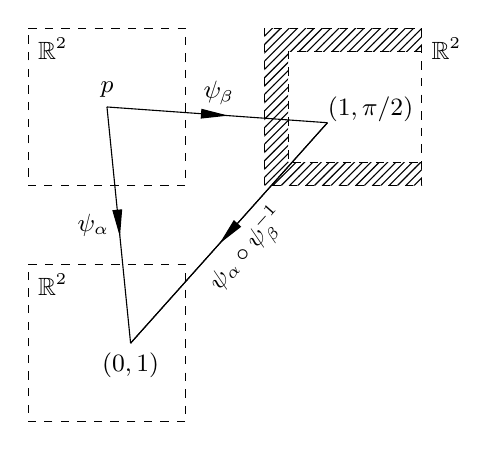
\begin{tikzpicture}[decoration={markings,mark=at position 0.55 with {\arrow{>}} },scale=1]
        \draw[dashed] (-1,1) node[below right]{\small$\mathbb{R}^2$}--(1,1)--(1,-1)--(-1,-1)--cycle;
        \draw[dashed] (4,1) node[below right]{\small$\mathbb{R}^2$}--(4,-1)--(2,-1)--(2,1)--cycle;
        \draw[dashed] (-1,-2) node[below right]{\small$\mathbb{R}^2$}--(1,-2)--(1,-4)--(-1,-4)--cycle;
        \fill[pattern=north east lines] (4,0.7)--(2.3,0.7)--(2.3,-0.7)--(4,-0.7)--(4,-1)--(2,-1)--(2,1)--(4,1);
        \draw[dashed] (4,0.7)--(2.3,0.7)--(2.3,-0.7)--(4,-0.7);
        \draw[postaction={decorate}] (0,0)node[above]{\small$p$}--(0.3,-3)  node[midway,left]{\small$\psi_\alpha$};
        \draw[postaction={decorate}] (2.8,-0.2)--(0.3,-3) node[below]{\small$(0,1)$};
        \draw (0.3,-3)--(2.8,-0.2) node[midway,sloped,below]{\small$ \psi_\alpha\circ\psi_\beta^{-1}$};
        \draw[postaction={decorate}] (0,0)--(2.8,-0.2) node[above right,inner sep=0pt]{\small$(1,\pi/2)$} node[midway,sloped,above]{\small$ \psi_\beta$};
    \end{tikzpicture}



\end{document}